\section{Discrete Random Variables}

A \emph{random variable} $X$ is a function $X : \Omega \implies \Re$
that maps an outcome $\epsilon \in \Omega$ to a number $X(\epsilon)$ on the real line.
We call it a variable because it has multiple states.

The \emph{expectation} of a random variable $X$ is
\begin{equation}
    E[X] = \sum_{x\in X(\Omega)} xp_X(x)
\end{equation}
The difference between $E[X]$ and the mean is
that $E[X]$ is computed from the ideal histogram,
while mean is computed from the empirical histogram.
In general for any functions $g$ and $h$,
\begin{align}
    E[g(X)]        & = \sum_{x} g(x)p_X(x) \\
    E[g(X) + h(X)] & = E[g(X)] + E[h(X)]   \\
    E[cX]          & = cE[X]               \\
    E[X + c]       & = E[X] + c
\end{align}

The \emph{variance} of a random variable $X$ is
\begin{equation}
    Var[X] = E\left[(X-\mu)^2\right]
\end{equation}
or alternatively, the second moment
minus the first moment squared.
\begin{equation}
    E[X^2] - E[X]^2
\end{equation}

The \emph{probability mass function} (PMF) $p_X(a)$
of a random variable $X$ specifies the probability of
obtaining a number $X(\epsilon) = a$. We denote a PMF as
\begin{equation}
    p_X(a) = P[X = a]
\end{equation}
PMFs are represented with histograms.
\begin{figure}[h]
    \centering
    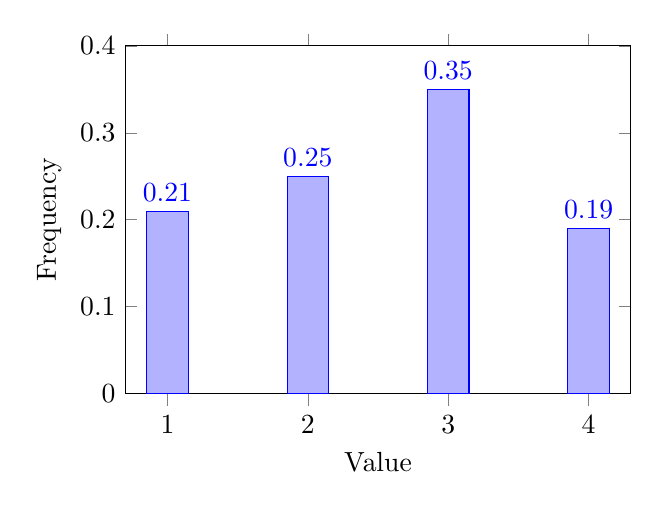
\begin{tikzpicture}
        \begin{axis}[
                ybar,
                bar width=15pt,
                xlabel={Value},
                ylabel={Frequency},
                xtick=data,
                ymin=0,
                ymax=0.4,
                nodes near coords,
                width=8cm,
                height=6cm
            ]
            \addplot coordinates {(1,0.21) (2,0.25) (3,0.35) (4,0.19)};
        \end{axis}
    \end{tikzpicture}
    \caption{PMF}
\end{figure}
A PMF should satisfy
\begin{equation}
    \sum_{x\in X(\Omega)} p_X(x) = 1
\end{equation}

The \emph{cumulative distribution function} is given by
\begin{align}
    F_X(x) & = P\left[X \leq x\right] \\
           & = \sum_{u \leq x} p_X(u)
\end{align}
and represents the sum of every impulse
of the PMF up to $x$.

A \emph{Bernoulli random variable} has a state
of either 0 or 1. The probability of getting 1 is $p$ and
the probability of getting 0 is $1 - p$. We write
\begin{equation}
    X \sim Bernoulli(p)
\end{equation}
or
\begin{equation}
    X \sim B(p)
\end{equation}
to say that $X$ is drawn from a Bernoulli distribution
with a parameter $p$. For a Bernoulli distribution,
\begin{align}
    E[X]   & = p        \\
    E[X^2] & = p        \\
    Var[X] & = p(1 - p)
\end{align}
Say $S \sim B(1-p)$.
Let
\begin{align}
    P(R=0|S=0) & = 1 - \epsilon_0 \\
    P(R=1|S=0) & = \epsilon_0
\end{align}
then $R|S=0 \sim B(\epsilon_0)$.
Let
\begin{align}
    P(R=0|S=1) & = \epsilon_1     \\
    P(R=1|S=0) & = 1 - \epsilon_1
\end{align}
then $R|S=0 \sim B(1 - \epsilon_1)$.
Overall,
\begin{equation}
    R|S \sim B(\epsilon_0^{1-S}(1-\epsilon_1)^S)
\end{equation}

A \emph{Rademacher random variable} has two states, -1 and 1.
The probability of getting each is 0.5.

A \emph{binomial random variable} has a PMF of
\begin{equation}
    p_X(k) = {n\choose k} p^k (1 - p)^{n - k}, k = 0, 1, \dots n
\end{equation}
where $0 < p < 1$ is the binomial parameter, and $n$ is the total
number of states. We write
\begin{equation}
    X \sim Binomial(n, p)
\end{equation}
to say that $X$ is drawn from a binomial distribution with a
parameter $p$ of size $n$.
If $X \sim Binomial(n, p)$, then
\begin{align}
    E[X]   & = np               \\
    E[X^2] & = np(np + (1 - p)) \\
    Var[X] & = np(1 - p)
\end{align}

Let $X$ be a \emph{geometric random variable}. Then the
PMF of $X$ is
\begin{equation}
    p_X(k) = (1 - p)^{k - 1}p, k=1,2,\dots
\end{equation}
We write
\begin{equation}
    X \sim Geometric(p)
\end{equation}
to say that $X$ was drawn from a geometric
distribution with a parameter $p$.
If $X \sim Geometric(p)$ then
\begin{align}
    E[X]   & = \frac{1}{p}                 \\
    E[X^2] & = \frac{2}{p^2} - \frac{1}{p} \\
    Var[X] & = \frac{1 - p}{p^2}
\end{align}

Let $X$ be a \emph{Poisson random variable}. Then the PMF
of $X$ is
\begin{equation}
    p_X(k) = \frac{\lambda^k}{k!}e^{-\lambda}, k=0, 1, 2,\dots
\end{equation}
where $\lambda > 0$ is the Poisson rate. We write
$X \sim Poisson(\lambda)$ to say that $X$ was drawn from
a Poisson distribution with a parameter $\lambda$.
If $X \sim Poisson(\lambda)$ then
\begin{align}
    E[X]   & = \lambda             \\
    E[X^2] & = \lambda + \lambda^2 \\
    Var[X] = \lambda
\end{align}
For small $p$ and large $n$,
\begin{equation}
    {n\choose k}p^k(1-p)^{n-k} \approx \frac{\lambda^k}{k!}e^{-\lambda}
\end{equation}

\emph{Joint Distributions} are higher-dimensional
PDFs, PMFs, or CDFs. We write
\begin{equation}
    f_{X_1, X_2, \dots, X_n}(x_1, x_2, \dots, x_n) \equiv f_{\vec{X}}(\vec{x})
\end{equation}

The \emph{joint PMF} of two random variables
$X$ and $Y$ is notated by
\begin{equation}
    p_{X,Y}(x,y)=P[X=x \text{ and } Y=y]
\end{equation}
and represents the probability of both.

A \emph{marginal PMF} is defined as
\begin{equation}
    p_X(x) = \sum_{y\in \Omega_Y} p_X(x,y)
\end{equation}
or w.l.o.g.
\begin{equation}
    p_Y(y) = \sum_{x\in \Omega_X} p_X(x,y)
\end{equation}
That is, it is the joint PMF summed over
one of the variables.

The \emph{conditional PMF} is given by
\begin{equation}
    p_{X|Y}(x|y) = \frac{p_{X,Y}(x,y)}{p_{Y}(y)}
\end{equation}

If two random variables $X$ and $Y$ are independent,
then
\begin{align}
    p_{X,Y}  & = p_X(x)p_Y(y) \\
    f_{X, Y} & = f_X(x)f_Y(y)
\end{align}
If a sequence of random variables
$X_1, X_2, \dots, X_N$ are independent,
then their joint PDF (or joint PMF) can be
factorized as
\begin{equation}
    f_{X_1,X_2,\dots,X_N}\left(x_1,x_2,\dots,x_N\right) = \prod_{n=1}^{N}f_{X_n}(x_n)
\end{equation}

The \emph{joint CDF} of two random variables
$X$ and $Y$ is the function $F_{X,Y}(x,y)$ such
that
\begin{equation}
    F_{X,Y}(x,y) = P\left[X \leq x \cap Y \leq y\right]
\end{equation}
If $X$ and $Y$ are discrete, then
\begin{equation}
    F_{X,Y}(x,y) = \sum_{y'\leq y}\sum_{x' \leq x} p_{X,Y}(x',y')
\end{equation}

For two random variables $X$ and $Y$,
the \emph{marginal CDF} is
\begin{align}
    F_X(x) & = F_{X,Y}(x, \infty) \\
    F_Y(y) & = F_{X,Y}(\infty, y)
\end{align}

Let $X$ and $Y$ be two random variables.
The \emph{joint expectation} is
\begin{equation}
    E[XY] = \sum_{y\in \Omega_Y}\sum_{x\in \Omega_X}xy \times p_{X,Y}(x,y)
\end{equation}
If $X$ and $Y$ are discrete, then joint
expectation is also called \emph{correlation}.
This can be written in matrix form as
\begin{equation}\label{eq:p}
    \begin{bmatrix}
        p_{X,Y}(x_1, y_1) & p_{X,Y}(x_1, y_2) & \dots  & p_{X,Y}(x_1, y_N) \\
        p_{X,Y}(x_2, y_1) & p_{X,Y}(x_2, y_2) & \dots  & p_{X,Y}(x_2, y_N) \\
        \vdots            & \vdots            & \ddots & \vdots            \\
        p_{X,Y}(x_N, y_1) & p_{X,Y}(x_N, y_2) & \dots  & p_{X,Y}(x_N, y_N)
    \end{bmatrix}
\end{equation}
then the joint expectation is
\begin{equation}
    E[XY] = \sum_{i=1}^{N}\sum_{j=1}^{N}x_i y_j \times p_{X,Y}(x_i, y_j)
\end{equation}
Let the matrix in Equation \ref{eq:p} be $\mathbf{P}$.
Let
\begin{align}
    \vec{x} & = \begin{bmatrix}
                    x_1    \\
                    x_2    \\
                    \vdots \\
                    x_N
                \end{bmatrix} \\
    \vec{y} & = \begin{bmatrix}
                    y_1    \\
                    y_2    \\
                    \vdots \\
                    y_N
                \end{bmatrix}
\end{align}
then
\begin{align}
    E[XY] & = \begin{bmatrix}
                  x_1   &
                  x_2   &
                  \dots &
                  x_N
              \end{bmatrix}
    \begin{bmatrix}
        p_{X,Y}(x_1, y_1) & p_{X,Y}(x_1, y_2) & \dots  & p_{X,Y}(x_1, y_N) \\
        p_{X,Y}(x_2, y_1) & p_{X,Y}(x_2, y_2) & \dots  & p_{X,Y}(x_2, y_N) \\
        \vdots            & \vdots            & \ddots & \vdots            \\
        p_{X,Y}(x_N, y_1) & p_{X,Y}(x_N, y_2) & \dots  & p_{X,Y}(x_N, y_N)
    \end{bmatrix}
    \begin{bmatrix}
        y_1    \\
        y_2    \\
        \vdots \\
        y_N
    \end{bmatrix}                         \\
          & = \vec{x}^T \mathbf{P} \vec{y}
\end{align}
$E[XY]$ is a weighted inner product between the
states. $\vec{x}$ and $\vec{y}$ are the states of
the random variables $X$ and $Y$. Recalling that the
magnitude of the inner product of $\vec{a}$ and $\vec{b}$
is $|a||b|\cos(\theta)$ and that cosine is bounded, we have
\begin{equation}
    -1 \leq \frac{E[XY]}{\sqrt{E[X^2]}\sqrt{E[Y^2]}} \leq 1
\end{equation}
Notice that the correlation of $X,Y$ is
proportional to the covariance.